% Example of a lycée pilote série in MIR rendering (4 exercises of the bank).
% Compile from the repo root, twice (for the sommaire):  TEXINPUTS=latex//: xelatex latex/examples/serie-pilote-enonce.tex
% Same file with \usepackage[level=1]{axiomath} (no "mir") = the coloured handout.
\documentclass[12pt,a4paper]{article}
\usepackage[level=1,mir]{axiomath}
\axsetup{title={Thalès et calcul numérique}, serie=3, classe={1\textsuperscript{ère} année -- lycée pilote}}
\begin{document}
\axmaketitle
\sommaire
\begin{rappels}
\emph{Thalès.} Si $M\in(AB)$, $N\in(AC)$ et $(MN)\parallel(BC)$, alors $\dfrac{AM}{AB}=\dfrac{AN}{AC}=\dfrac{MN}{BC}$ ;
réciproquement, si $\dfrac{AM}{AB}=\dfrac{AN}{AC}$ et si les points sont dans le même ordre, $(MN)\parallel(BC)$.
\emph{Racines.} Pour $a\geq0$, $b>0$ : $\sqrt{ab}=\sqrt a\,\sqrt b$ et $\sqrt{a/b}=\sqrt a/\sqrt b$ ; on rend un dénominateur
rationnel avec la quantité conjuguée.
\end{rappels}
\begin{exo}[title={Aires dans un trapèze}, stars=4]
$ABCD$ est un trapèze de bases $[AB]$ et $[DC]$, avec $AB=a<DC=b$. Ses diagonales se coupent en $O$. On note $S_1$, $S_2$, $S_3$ et $S_4$ les aires des triangles $OAB$, $OCD$, $OAD$ et $OBC$.

\begin{center}
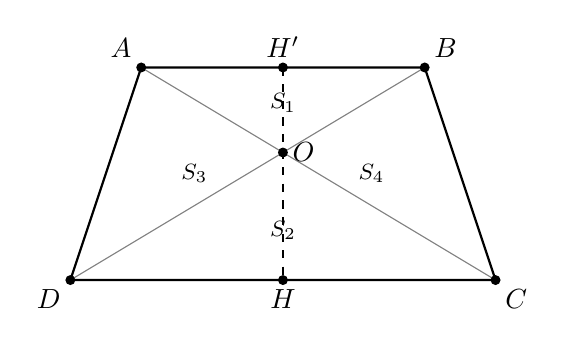
\begin{tikzpicture}[scale=0.9]
  \coordinate (D) at (0,0); \coordinate (C) at (6,0); \coordinate (A) at (1,3); \coordinate (B) at (5,3); \coordinate (O) at (3,1.8);
  \coordinate (H) at (3,0); \coordinate (Hp) at (3,3);
    \draw[thick] (A)--(B)--(C)--(D)--cycle; \draw[gray] (A)--(C); \draw[gray] (B)--(D); \draw[dashed] (Hp)--(H);
  \foreach \p/\pos in {A/above left,B/above right,C/below right,D/below left,O/right,H/below}{\fill (\p) circle (2pt) node[\pos]{$\p$};}
  \fill (Hp) circle (2pt) node[above]{$H'$};
  \node at (3,2.5) {\footnotesize$S_1$}; \node at (3,0.7) {\footnotesize$S_2$}; \node at (1.75,1.5) {\footnotesize$S_3$}; \node at (4.25,1.5) {\footnotesize$S_4$};
\end{tikzpicture}
\end{center}
\begin{enumerate}
  \item Montrer que $\dfrac{OA}{OC}=\dfrac{OB}{OD}=\dfrac ab$.
  \item La perpendiculaire à $(AB)$ passant par $O$ coupe $(AB)$ en $H'$ et $(DC)$ en $H$. Montrer que $\dfrac{OH'}{OH}=\dfrac ab$, puis que $\dfrac{S_1}{S_2}=\dfrac{a^2}{b^2}$.
  \item Montrer que $S_3=S_4$. [Comparer les aires de $ABD$ et de $ABC$.]
  \item Montrer que $\dfrac{S_3}{S_1}=\dfrac ba$, puis que $S_3^{\,2}=S_1\,S_2$.
  \item En déduire que l'aire du trapèze est $\big(\sqrt{S_1}+\sqrt{S_2}\big)^2$.
  \item Application : $S_1=16$ et $S_2=25$. Calculer $S_3$, l'aire du trapèze et le rapport $\dfrac ab$.
\end{enumerate}
\end{exo}

\begin{exo}[title={Une droite par le centre de gravité}, stars=4]
$ABC$ est un triangle, $I$ le milieu de $[BC]$ et $G$ le point de $[AI]$ tel que $AG=\dfrac23AI$. Une droite $d$ passant par $G$, mais pas par $A$, coupe $[AB]$ en $M$ et $[AC]$ en $N$. Les parallèles à $d$ passant par $B$ et par $C$ coupent la droite $(AI)$ en $U$ et $V$ ; on admet que $U$ et $V$ sont sur la demi-droite $[AI)$, au-delà de $G$.

\begin{center}
\begin{tikzpicture}[scale=1.15]
  \coordinate (A) at (3,6); \coordinate (B) at (0,0); \coordinate (C) at (9,0); \coordinate (I) at (4.5,0); \coordinate (G) at (4,2);
  \coordinate (M) at (0.75,1.5); \coordinate (N) at (6.6,2.4); \coordinate (U) at (4.3333,0.6667); \coordinate (V) at (4.6667,-0.6667);
  \draw[thick] (A)--(B)--(C)--cycle; \draw[gray] (A)--(V);
  \draw[thick] ($(M)!-0.35!(N)$)--($(N)!-0.25!(M)$);
  \draw[dashed] (B)--(U); \draw[dashed] (C)--(V);
  \foreach \p/\pos in {A/above,B/below left,C/below right,I/above left,G/above left,M/left,N/right,U/above right,V/below right}{\fill (\p) circle (2pt) node[\pos]{$\p$};}
  \node[axmain] at (-0.55,1.25) {$d$};
\end{tikzpicture}
\end{center}
\begin{enumerate}
  \item Montrer que $I$ est le milieu de $[UV]$, puis que $AU+AV=2\,AI$. [Papillon de sommet $I$ dans les triangles $IBU$ et $ICV$.]
  \item Écrire Thalès de sommet $A$ dans les triangles $ABU$ et $ACV$ pour montrer que $\dfrac{AB}{AM}=\dfrac{AU}{AG}$ et $\dfrac{AC}{AN}=\dfrac{AV}{AG}$.
  \item En déduire que $\dfrac{AB}{AM}+\dfrac{AC}{AN}=3$.
  \item Application : $AB=12$, $AC=10$ et $AM=9$. Calculer $AN$. Que devient la relation lorsque $d\parallel(BC)$ ? lorsque $d=(BG)$ ?
  \item On pose $x=\dfrac{AM}{AB}$, $y=\dfrac{AN}{AC}$ et on note $\mathcal S$ l'aire de $ABC$. Montrer que $\text{aire}(AMN)=xy\,\mathcal S$, puis que $\dfrac49\,\mathcal S\leq\text{aire}(AMN)\leq\dfrac12\,\mathcal S$. Préciser les positions de $d$ pour lesquelles il y a égalité. [Poser $u=\dfrac1x$ ; montrer que $1\leq u\leq2$ et que $xy=\dfrac1{u(3-u)}$.]
\end{enumerate}
\end{exo}

\begin{exo}[title={Racines irrationnelles}, stars=4]
Un nombre est \emph{rationnel} s'il s'écrit $\dfrac pq$ avec $p$, $q$ entiers, $q\neq0$, la fraction étant irréductible ($p$ et $q$ n'ont pas de diviseur commun autre que $1$).
\begin{enumerate}
  \item Montrer que si le carré d'un entier $n$ est pair, alors $n$ est pair. [Étudier le cas $n$ impair.]
  \item On suppose que $\sqrt2=\dfrac pq$ (fraction irréductible). Montrer que $p^2=2q^2$, puis que $p$ et $q$ sont pairs. Conclure que $\sqrt2$ n'est pas rationnel.
  \item Montrer de même que $\sqrt6$ n'est pas rationnel.
  \item En calculant $(\sqrt2+\sqrt3)^2$, montrer que $\sqrt2+\sqrt3$ n'est pas rationnel.
  \item En déduire que $\sqrt3-\sqrt2$ n'est pas rationnel.
\end{enumerate}
\end{exo}

\begin{exo}[title={PGCD et divisibilité par 2, 4, 8}, stars=4]
Pour tout entier naturel $n$, on pose $d_n=\mathrm{PGCD}(n+2,\ n^2+4)$.
\begin{enumerate}
  \item Calculer $d_n$ pour $n=0,1,2,\dots,8$.
  \item Montrer que $n^2+4=(n+2)(n-2)+8$. En déduire que $d_n=\mathrm{PGCD}(n+2,\ 8)$.
  \item Montrer que $d_n=1$ si $n$ est impair, $d_n=2$ si $n$ est multiple de $4$, $d_n=4$ si $n=8q+2$ et $d_n=8$ si $n=8q+6$.
  \item Calculer $d_{2026}$ et $d_{2030}$.
\end{enumerate}
\end{exo}

\end{document}
